\chapter{\chImplementation}
\label{ch:implementation}

\newcontent{
    After reviewing the existing benchmarking tools, we consider improving the situation to fulfill our requirements.
    At first, \first~tried refactoring a fork of \textsc{benchmark-tool}\footlink{https://github.com/daajoe/benchmark-tool/tree/refactor}.
    We improved the tool architecture to be more decentralized, allowing the benchmark to be shared easily.
    We has also written documentation and getting started guide for this tool.
    But after those efforts, we decided to create a new tool instead.
    This is because to create the ideal tool, we need significant architecture overhaul and decided it is better to start anew.
}

This chapter discusses the design and implementation of \OurBenchmarkingTool, a new benchmarking tool developed to address the requirements defined in Section \ref{sec:idealBenchmarkingTool}.
Section \ref{sec:impl.design} will describe the system design and the reason behind the design decisions.
The chapter will then conclude with a description about the implementation in Section \ref{sec:impl.impl}.


\section{Preliminary}
\label{sec:impl.prelim}

% \First~also take some ideas from the existing tools.
% For example, \first~take the approach of \textsc{JuBE} that presents wide range of extensibility and is agnostic to the resource monitoring tool used for the benchmark.
% Modular approach used in \textsc{compbench} is also interesting to take as it provides easy implementation of extensibility.
% We integrate these ideas to our own approach such as the \textsc{client-server} architecture.



\section{System Design}
\label{sec:impl.design}

This section discusses the design of \OurBenchmarkingTool~and its rationale.
This includes the system architecture, messaging mechanism, and also the workflow and model of benchmarking.

\subsection{Architecture}
\label{sec:impl.architecture}

\begin{figure}
    \centering
    \ifdraft{
        \dummyfig{assets/diagrams/arch.tikz}
    }{
        \makeatletter
\tikzset{
    database/.style={
        path picture={
            \draw (0, 1.5*\database@segmentheight) circle [x radius=\database@radius,y radius=\database@aspectratio*\database@radius];
            \draw (-\database@radius, 0.5*\database@segmentheight) arc [start angle=180,end angle=360,x radius=\database@radius, y radius=\database@aspectratio*\database@radius];
            \draw (-\database@radius,-0.5*\database@segmentheight) arc [start angle=180,end angle=360,x radius=\database@radius, y radius=\database@aspectratio*\database@radius];
            \draw (-\database@radius,1.5*\database@segmentheight) -- ++(0,-3*\database@segmentheight) arc [start angle=180,end angle=360,x radius=\database@radius, y radius=\database@aspectratio*\database@radius] -- ++(0,3*\database@segmentheight);
        },
        minimum width=2*\database@radius + \pgflinewidth,
        minimum height=3*\database@segmentheight + 2*\database@aspectratio*\database@radius + \pgflinewidth,
    },
    database segment height/.store in=\database@segmentheight,
    database radius/.store in=\database@radius,
    database aspect ratio/.store in=\database@aspectratio,
    database segment height=0.1cm,
    database radius=0.25cm,
    database aspect ratio=0.35,
}
\makeatother

\tikzstyle {block} = [draw, text width=4cm, minimum height=1cm, align=center]
\tikzstyle {miniblock} = [draw=gray, dashed, text width=3cm, inner sep=1ex]

\begin{tikzpicture}
    \node [block] (bootstrapper) {Bootstrapper};
    \node [block, below=of bootstrapper] (manager) {Manager};
    \node [block, below=1.5cm of manager, inner sep=0pt] (worker) {
        \begin{tikzpicture}
            \matrix [row sep=1em] {
                \node {Worker}; \\
                \node [miniblock] {\footnotesize Collect System Info}; \\
                \node [miniblock] {\footnotesize Execute run}; \\
                \node [miniblock] {\footnotesize Validate result}; \\
                \node {\dots}; \\
            };
        \end{tikzpicture}
    };
    \draw [-latex'] (manager) -- (worker) node [midway, fill=white] {manages};

    \node [block, right=3cm of bootstrapper] (server) {Server};
    \node[database,database radius=0.5cm,database segment height=0.3cm, below=of server] (database) {};
    \node [right=0.1cm of database] {\rotatebox{-90}{Database}};
    \node [block, below=of database, inner sep=0pt] (analyzer) {
        \begin{tikzpicture}
            \matrix [row sep=1em] {
                \node {Analyzer}; \\
                \node [miniblock] {\footnotesize Summarize runtime}; \\
                \node [miniblock] {\footnotesize Cactus plot}; \\
                \node {\dots}; \\
            };
        \end{tikzpicture}
    };
    \draw (server) -- (database);
    \draw (database) -- (analyzer);

    \draw [-latex'] (bootstrapper) -- (server) node [midway, fill=white] {$R \in C \times I$};
    \path [-latex', transform canvas={xshift=-0.1cm}] (server) edge node [sloped, above, pos=0.33, fill=white] {$(c,i) \in R$} (worker);
    \path [-latex', transform canvas={xshift=0.1cm}] (worker) edge node [sloped, below, pos=0.33, fill=white] {reports to} (server);

    \begin{scope}[on background layer]
        \node[draw=red!50, dashed, inner sep=1ex, label=above:\sffamily\textsc{client-side},  rounded corners, fit=(bootstrapper)(manager)(worker)] (clientenv) {};
        \node[draw=blue!50, dashed, inner sep=1ex, label=above:\sffamily\textsc{server-side},  rounded corners, fit=(server)(database)(analyzer)] (serverenv) {};
        \path [draw=black!30, dashed] ([xshift=1.5cm] clientenv.north east) edge node [sloped, near end, text=black!60, fill=white] {TCP} ([xshift=1.5cm] clientenv.south east);
    \end{scope}

\end{tikzpicture}

    }
    \caption{Architecture of \OurBenchmarkingTool}
    \label{fig:architecture}
\end{figure}

Figure \ref{fig:architecture} shows the architecture of \OurBenchmarkingTool, our attempt on a new benchmarking tool fulfilling most of the defined requirements.
The architecture follows the client-server design pattern, communicating through Transmission Control Protocol (TCP).
The client manages the heavy computation while the server manages the data.
Typically, the client will be in a high performance computing (HPC) cluster system while the server in a separate system, e.g. a virtual private server (VPS).

This decision to use client-server architecture is made to handle concurrent writes to the database, which is difficult to achieve in some database engines.
With a single server process to manage the database, the writes can be queued in the application level.
This provides a clean separation of computation and data.

Furthermore, the server can be separated to another system outside of the cluster system, allowing avoidance of filesystem-related issues such as locking issues on NFS (Network File System).
Long running job is arguably an anti-pattern in job scheduling, because not only it will take a long time before it's scheduled, it will also prevent other jobs from being scheduled.

\emph{Server} manages the data in the database.
It receives events through a TCP socket and optionally send replies.
To achieve extensibility, the server maintains a specified set of \emph{observers}, each listening for related events.
The events are distributed through a publisher-subscriber design pattern.
The observer will then executes its jobs, such as inserting data to the database.

\emph{Bootstrapper} is a component that will read the configuration file from the user, prepare the computing environment, and then tell the server $R \in C \times I$, the set of benchmark runs that will be executed.
Among the things prepared are the tools, benchmark instances, and database schema.
Preparing the specified tools and instances may additionally include downloading and running related setting up steps.
In short, the bootstrapping is also separated to the computation-related and data-related between the client-side and server-side.

\emph{Manager} manages the benchmark workers.
This component acts as an interface to the underlying job submitting system, or even implements its own job queue as in the case of the \emph{local} manager.
Manager will first ask for a list of pending runs from the server before assigning the runs to workers.
The manager is responsible for deploying, assigning tasks, and stopping the benchmark workers, making sure they finishes the assigned job.
This allows the benchmarking tool to be agnostic about the execution environment and can be extended in many ways.

\emph{Workers} do the heavy computing steps, typically in parallel.
Because the benchmark run is embarrassingly parallel\footnote{there is no effort needed to parallelize the problem since there is no dependencies between tasks}, each worker can be run as its own process without interacting with other workers.
Submitted to a HPC cluster, this allows the computation to be executed as fast as possible.
A worker is assigned a run identifier and executes the needed steps for the benchmark run after asking the context (i.e. $r = (c, i) \in R$) from the server.

A worker consists of smaller building blocks called \emph{run steps}.
The run step is executed in sequence.
In most cases, one of these steps, called the \emph{executor}, acts as a resource monitor and executes the tool configuration $c$ with the instance $i$.
The executor then measures and limits the execution of the tool.
Finally, each step can report its result to the server.

The worker only executes one specific benchmark run as opposed to requesting many jobs as its available.
This is also to prevent worker to be a long-running job.
A worker maps nicely to a job in the HPC cluster system.

\emph{Analyzer} aggregates the data from the database and analyze it, outputting a presentable result.
This component is usually used after the benchmarking is finished, but it can also be used to serve a live analysis of a benchmarking in process.
Analyzer also consists of steps that is implemented as a modular, reusable module.
This is to encourage code reuse and minimize the effort of doing the common analysis of research results.


\subsection{Messaging}
\label{sec:impl.messaging}

\begin{figure}
    \ifdraft{
        \dummyfig{assets/diagrams/zeromq.tikz}
    }{
        \usetikzlibrary{shapes,arrows,positioning,fit,backgrounds}

\tikzstyle{bidirectional} = [draw, latex'-latex', line width=1.15pt]

\tikzset{
    pics/zmq2/.style n args = {3}{
        code = {
        \node[fill=white, minimum height=3em, align=center, text width=9em] (-A) at (0,0) {#1};
        \node[fill=black!5, anchor=north east, text width=4em, align=center] (-B) at (-A.south) {\textsc{#2}};
        \node[fill=black!5, anchor=north west, text width=4em, align=center] (-C) at (-A.south) {\textsc{#3}};
        \node[inner sep=0pt,draw,rounded corners,fit=(-A)(-B)(-C)] {};
        \draw (-B.north west) -- (-C.north east)
              (-B.north east) -- (-C.south west);
        }
    },
    pics/zmq1/.style n args = {2}{
        code = {
        \node[fill=white, minimum height=3em, align=center, text width=5em] (-A) at (0,0) {#1};
        \node[fill=black!5, anchor=north, text width=5em, align=center] (-B) at (-A.south) {\textsc{#2}};
        \draw (-B.north west) -- (-B.north east);
        \node[inner sep=0pt,draw,rounded corners,fit=(-A)(-B)] {};
        }
    },
}


\resizebox{\textwidth}{!}{%
    \begin{tikzpicture}
        \node (workerdots) {\huge\vdots};
        \pic [above=of workerdots, local bounding box=worker2] (w2) {zmq1={Worker 2}{dealer}};
        \pic [above=2cm of worker2, local bounding box=worker1] (w1) {zmq1={Worker 1}{dealer}};
        \pic [below=of workerdots, local bounding box=workern] (wn) {zmq1={Worker $n$}{dealer}};

        \pic [right=3cm of workerdots, local bounding box=server] (s) {zmq2={Gateway}{router}{pub}};

        \node [right=3cm of server] (observerdots) {\huge\vdots};
        \pic [above=of observerdots, local bounding box=observer2] (o2) {zmq1={Observer 2}{sub}};
        \pic [above=of observer2, local bounding box=observer1] (o1) {zmq1={Observer 1}{sub}};
        \pic [below=of observerdots, local bounding box=observern] (on) {zmq1={Observer $n$}{sub}};

        \draw [bidirectional] (w1-B.east) -- (s-B.west);
        \draw [bidirectional] (w2-B.east) -- (s-B.west);
        \draw [bidirectional] (wn-B.east) -- (s-B.west);

        \draw [bidirectional] (s-C.east) -- (o1-B.west);
        \draw [bidirectional] (s-C.east) -- (o2-B.west);
        \draw [bidirectional] (s-C.east) -- (on-B.west);

        \node [inner sep=.5cm, text=red!60!black, above, rotate=90, text width=4em] (w1label) at (worker1.west) {\sffamily\textsc{worker process}};
        \node [inner sep=.5cm, text=red!60!black, above, rotate=90, text width=4em] (w2label) at (worker2.west) {\sffamily\textsc{worker process}};
        \node [inner sep=.5cm, text=red!60!black, above, rotate=90, text width=4em] (wnlabel) at (workern.west) {\sffamily\textsc{worker process}};


        \begin{scope}[on background layer]
            \node[fit=(worker1)(worker2)(workerdots)(workern)] (workers) {};
            \node[fit=(observer1)(observer2)(observerdots)(observern)] (observers) {};

            \node[fill=red!5, rounded corners, fit=(worker1)(w1label)] {};
            \node[fill=red!5, rounded corners, fit=(worker2)(w2label)] {};
            \node[fill=red!5, rounded corners, fit=(workern)(wnlabel)] {};
            \node[fill=blue!5, rounded corners, fit=(server)(observers)] (serverenv) {};
        \end{scope}

        \node [inner sep=.5cm, text=blue!60!black, below right] at (serverenv.north west) {\sffamily\textsc{server process}};


    \end{tikzpicture}
}
    }
    \caption{Messaging architecture of \OurBenchmarkingTool}
    \label{fig:zmq}
\end{figure}

Figure \ref{fig:zmq} gives an overview of the messaging architecture and the overall network of \OurBenchmarkingTool.
Each process is independent to each other and can be separated across virtual nodes.
This means it can be implemented in a single node, in a cluster system, or even across clusters.
Data is transported through TCP for inter-process communication, and through local in-process (inter-thread) transportation for intra-process communication.
Communication follows some basic messaging patterns used by the \O MQ (ZeroMQ)\footlink{http://zeromq.org/} messaging framework, namely \textsc{router-dealer} and \textsc{pub-sub}.

\First~decided to use \O MQ to avoid reinventing the wheel and just focus on the core functionalities.
\O MQ provides many messaging patterns for many use cases.
It is also lightweight and easily available in most platform with a lot of supported languages.

The \textsc{router-dealer} patterns allows two-way communication between the party \citep{hintjens2013zeromq}.
This is used in the communication between the worker and the server gateway.
The patterns allows many workers to send events to the server and optionally request for a reply from the server.
The message sent to a \textsc{router} socket is enveloped by a unique identifier, allowing the \textsc{router} to reply to the correct \textsc{dealer}.
This powerful pattern allows reliable many to one communication between the workers and the server gateway.

On the other hand, \textsc{pub-sub} patterns follows the publisher-subscriber pattern as its name suggests \citep{hintjens2013zeromq}.
This is a fan-out pattern, on which the publisher just publish the message without caring if the message is received.
Both the publisher and subscriber does not know each other.
The \textsc{pub} socket just publish the message to the socket, and the \textsc{sub} sockets listen to one or more `topics'.
This allows fast distribution of event message received by the server gateway to the possibly many observers.
The downside is the distribution is not reliable since the message is just thrown without confirmation if the other party is ready.
This can be corrected with proper synchronization using other messaging pattern if needed.


\subsection{Benchmarking Workflow}
\begin{figure}
    \centering
    \ifdraft{
        \dummyfig{assets/pics/workflow-swimlane.png}
    }{
        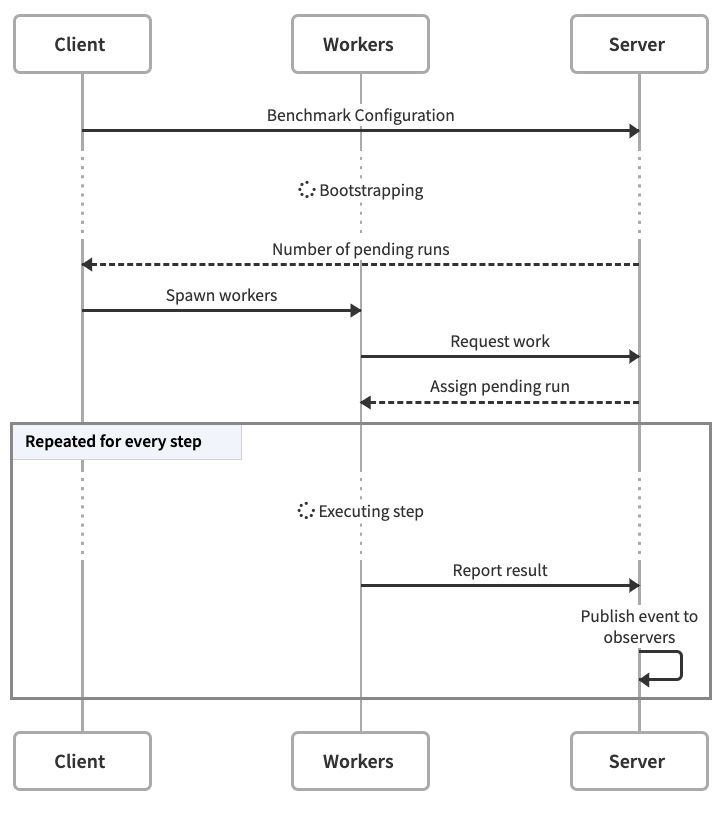
\includegraphics[width=\textwidth]{assets/pics/workflow-swimlane.png}
    }
    \caption{Benchmarking workflow}
    \label{fig:swimlane}
\end{figure}

Figure \ref{fig:swimlane} presents the steps and interactions taken by each actors, namely the Client, Workers, and Server.
Aside from the already defined Workers and Server in Section \ref{sec:impl.architecture} above, Client represents the actual user interfacing with \OurBenchmarkingTool.
Note that the figure assumes the server is already started.

First, the client uses the bootstrapper to read the configuration and then send a bootstrap event to the server.
This event includes the needed information for the server to also set up the database schema.
Then the server replies its readiness to the client.
After that, the client uses the manager to spawn workers.
This is the end of the interaction needed by the user.

Then, after being scheduled by the job scheduling system used by the manager, each worker request the context for its assigned run identifier to the server.
The server replies with the context.
This includes things such as the tool and its configuration, the input instance, resource limits, etc.

Then come the main computation represented as run steps.
Each steps is executed sequentially.
After execution of the step, typically the worker will report the result to the server which in turn publish that event to observers.
Any observers listening to the event will execute its work, often time this means inserting data to the database. After there is no more run step to execute, the worker sends a finish event to the server and terminates.

As soon as soon as the bootstrapping is done, analysis can be executed from the available data in database.
This allows the flexibility of doing either on-demand analysis or live analysis.


\subsection{Benchmarking Model}

\First~decided to define the data as relational model of SQL, as opposed to nonrelational model of NoSQL.
The reason is because SQL provides an easy and fast interface for querying and aggregating data, tasks that occur often when analyzing benchmark results.
The benchmarking process itself can be defined nicely into structured relations, centering on benchmark runs.

\begin{figure}
    \centering
    \ifdraft{
        \dummyfig{assets/pics/erd.png}
    }{
        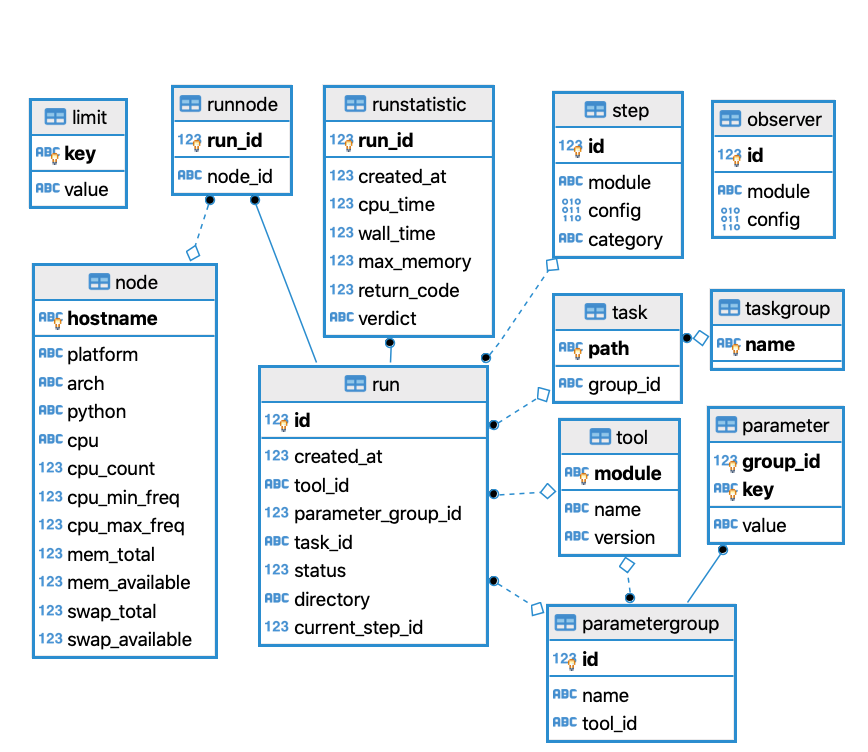
\includegraphics[width=\textwidth]{assets/pics/erd.png}
    }
    \caption{Entity-relationship diagram of \OurBenchmarkingTool's model}
    \label{fig:erd}
\end{figure}

The benchmarking process is modeled as in the entity-relationship diagram (ERD) shown in Figure \ref{fig:erd}.
The database stores every configuration defined to support reproducibility.
Among the core entities are \textsc{run}, \textsc{tool}, \textsc{parameter}, \textsc{limit}, \textsc{step}, \textsc{observer}, and \textsc{task}.
Some entities like \textsc{parameter} and \textsc{task} are grouped to another intermediate many-to-many entity, that is \textsc{parameterGroup} and \textsc{taskGroup}.
It can be seen that the relationship centers around the \textsc{run} entity.

Other modules, like the ones used as steps, can then register its own model to store its data, such as \textsc{runstatistic} (by the executor module) or \textsc{runnode} (by the system information collector module).
This supports separation of concern and encapsulation of the module.
User can use community-created module without having to consider its data model.

In fact, it is also possible to move all the data that is normally stored in the filesystem into the SQL table.
Many SQL database engine provides a BLOB data type to store binary data.
For example, \textsc{SQLite} even has an archiving tool called \code{sqlar}\footlink{https://www.sqlite.org/sqlar} that use the database as storage just like a ZIP archive.
This allow the database to store everything needed to reproduce the benchmark.
But \first~decided not to do it to make debugging runs easier, a task which also occur surprisingly often alongside benchmarking.

\section{Implementation}
\label{sec:impl.impl}

\newstyle{
This section presents details regarding the implementation of \OurBenchmarkingTool.
It will be organized by the components of the benchmarking tool.
The complete implementation source code is attached in the appendix.
It is also available as Git repository: \href{https://github.com/rkkautsar/reprobench}{\code{https://github.com/rkkautsar/reprobench}} and pypi package: \href{https://pypi.org/project/reprobench/}{\code{https://pypi.org/project/reprobench/}}.
}

\subsection{Development Environment}

\First~choose Python as the main programming language.
Specifically, Python 3 is used as its predecessor Python 2 will meet its end of the line and not be supported anymore in 2020.
It is a widely available language with huge community.
Python also has good interopability with C and C++, it's relatively easy to write wrappers of C libraries to Python.
That said, there is a huge collection of publicly available python packages in the Python Package Index (pypi)\footlink{https://pypi.org/} readily installable through \code{pip} tool, which often distributed alongside Python.
This allows for rapid software development by reducing common implementation.

Being an interpreter and not a compiled language, Python is relatively slow.
For this project, speed can be sacrificed in place of developer experience.
Most of the CPU usage will be used by the benchmarked program anyway, so the development speed is arguably more important.

\First~use a combination of \textsc{pyenv}\footlink{https://github.com/pyenv/pyenv} and \textsc{poetry}\footlink{https://github.com/sdispater/poetry} to manage dependencies and package publishing.
With \textsc{pyenv}, it is easy to switch between specific versions of Python and also pin a project to use specific version of Python.
This allow reproducible development environment across machines without influence from other projects using different Python version.
Additionally, testing if the software works under specific version of Python is a trivial task.
\textsc{poetry} on the other hand, manages the dependencies in a virtual environment with version locking.
This allows separate, reproducible dependencies across projects.
\textsc{poetry} also provide simple API to package and publish the project to pypi.
Under a UNIX system, setting up both tools is easy and works without superuser privilege, as seen in \lst~\ref{lst:impl.setup.pyenv.poetry}.

\begin{listing}
    \begin{minted}{bash}
$ curl https://pyenv.run | bash
$ pyenv install "3.7.2"
$ pyenv global "3.7.2"
$ pip install poetry
    \end{minted}
    \caption{Setting up \textsc{pyenv} and \textsc{poetry}}
    \label{lst:impl.setup.pyenv.poetry}
\end{listing}

The source code is organized by the Git version control and made publicly available in GitHub.
This allows others to freely contribute to the project and also encourage them to also make their modules open-source.
Additionally, the source code is licensed under the MIT License to allow permissive usage.

\subsection{Project Structure}
\label{sec:impl.structure}

The source code organization and their brief descriptions is listed below:
\begin{itemize}
    \item \emph{examples/}\\
          This directory provides a collection of working usage benchmark examples demonstrating various features of the benchmarking tool.

    \item \emph{pyproject.toml}\\
          Configuration file describing the various dependencies used and the packaging options used for publishing purposes.

    \item \emph{reprobench/console/}\\
          This directory consists of the implementations of the command line interface (CLI), including the \code{reprobench} root command and related setup for the sub-commands.

    \item \emph{reprobench/core/}\\
          The core implementation of \OurBenchmarkingTool~is organized in this directory.
          This includes generic classes, database models, and implementation for the worker, server, bootstrapper, and analyzer components.

    \item \emph{reprobench/executors/}\\
          Implementations of the special run step doing the actual execution and monitoring of the tools and its input.
          This includes the accompanying observer, its database model and related events.

    \item \emph{reprobench/managers/}\\
          Implementations of the manager component and its CLI sub-commands under the \code{reprobench manage} sub-command, e.g. \code{reprobench manage local} or \code{reprobench manage slurm}.
          In the future, it is preferable for each manager to be separated into its own package.

    \item \emph{reprobench/statistics/}\\
          This directory consists of reference implementations of the analysis step modules.
          It is encouraged to implement analysis steps as separate packages and only put the most general ones in the main project.

    \item \emph{reprobench/task\_sources/}\\
          This directory consists of various implementation for extracting tasks from the configuration.
          Currently, this includes local filesystem sourced tasks, URL-based remote sourced tasks, and Digital Object Identifier (DOI) sourced tasks.

    \item \emph{reprobench/tools/}\\
          This directory implements some base classes to be extended for writing tool interfaces.
          It is also possible in the future to allow tools to be defined only from the configuration, further lowering the barrier for using this benchmarking tool.
          Writing tool interface is discussed in Section \ref{sec:impl.tools}.

    \item \emph{reprobench/utils.py}\\
          This file consists of various small utilities commonly used by the implementation.


\end{itemize}


\subsection{Configuration}

\begin{listing}
    \inputminted{yaml}{assets/listings/pseudocodes/config.yml}
    \caption{Example of \OurBenchmarkingTool~configuration file}
    \label{lst:impl.config.example}
\end{listing}

Configuration for a benchmark is done using a YAML file, provided to the bootstrapper.
An example configuration file is shown in \lst~\ref{lst:impl.config.example}.
\First~choose YAML file over other format because of it is readable and easy to edit by hand.
It is also widely adopted and implemented in various programming languages.
\First~also considered to use XML or JSON but find both to be harder to edit by hand.

``YAML Ain’t Markup Language'', recursively abbreviated to YAML, is a data serialization language designed to be human-friendly, portable between programming languages, and easy to use for every tasks \citep{ben2005yaml}.
While it's easy to understand at a glance, it has an arguably complex specification allowing for various use cases.
Avoiding its complexity, \first~choose to use \textsc{StrictYAML}\footlink{https://github.com/crdoconnor/strictyaml}, a relatively simple implementation of a small subset of the YAML specification.
\textsc{StrictYAML} also allows definition of a schema to provide type-safe parsing.
The schema for \OurBenchmarkingTool~configuration file is defined in \emph{reprobench/core/schema.py}.


\subsection{Module}

To enable high extensibility, many components of \OurBenchmarkingTool~is defined in a modular, reusable Python \emph{modules}.
What \first~define as a module is in fact just a Python class that can be imported by path strings.
For example, the path string \mintinline{python}{"my_package.my_folder.my_file.MyClass"} references the class \code{MyClass} in \emph{my\_folder/my\_file.py} (or \emph{my\_folder/my\_file/\_\_init\_\_.py}) file in the Python package \code{my\_package}.
This allows \OurBenchmarkingTool~to flexibly import user defined code, either it's in the working directory or installed through \code{pip}.


\subsection{Server}

\begin{listing}
    \inputminted{python}{assets/listings/pseudocodes/server.py}
    \caption{Pseudo-code of the server component}
    \label{lst:impl.server}
    % \captionof{listing}{Pseudo-code of the server component \label{lst:impl.server}}
\end{listing}

Pseudo-code for the server implementation is given in \lst~\ref{lst:impl.server}.
In short, the server is implemented in three main phases.
The first phase is setting up the database and sockets.
Then the server waits for a \textsc{bootstrap} event from the client, as mentioned in Section \ref{sec:impl.design} earlier.
As soon as the database is bootstrapped, the server query the needed observers and register the respective modules.
Finally, the server spawn `greenlets' of the observers and its own loop method and waited for them to terminate.

\textsc{greenlet}\footlink{https://github.com/python-greenlet/greenlet} is a Python package that provides the use of `greenlets'.
A greenlet is a lightweight pseudo-thread useful for concurrent programming.
In contrast with implicit context switching of native OS-level threads, greenlet explicitly context switches.
In short, it's a way of programmatically jump from one code frame to another, allowing thread-like behavior with minimal runtime overhead.
This fits to \firstposs~need of concurrency for controlling the flow in the server.

On the first phase, an \textsc{SQLite} database are initiated in the given output path.
\First~choose to use SQLite because it is most of the time already available in various platforms.
Even when it is not available, it can be installed easily with pre-compiled binaries or as a single-file C source code.
It is also works on a single file database, allowing easy distribution for reproducibility.
The \textsc{SQLite} database is opened in \emph{Write-ahead logging} mode to better handle concurrency.

Two socket connections are also prepared in this phase.
The official Python bindings for \O MQ, \textsc{pyzmq}\footlink{https://github.com/zeromq/pyzmq} is used to setup the related sockets.
These two sockets are \textsc{router} and \textsc{pub} as discussed in Section \ref{sec:impl.messaging}.
On one hand, the \textsc{router} socket acts as a `front-end' gateway and interacts with clients.
On the other hand, the \textsc{pub} socket interacts with the observer greenlets and acts as the `back-end' gateway.

Then the server waits for a bootstrap event from the client.
Events are encoded with \textsc{MessagePack}\footlink{https://msgpack.org/} binary serialization format to minimize the amount of data transferred.
It enters a loop waiting for the specific \textsc{bootstrap} event.
After receiving this event, the server prepare the database schema with the payload from the event.
Then the server loads the observer modules.
The list of observer modules is extracted from the database, inserted from the earlier bootstrapping process.

The server spawns greenlets of the observers and its own loop method.
The loop method waits for every event received in the front-end socket and forward it to the back-end socket, allowing the observers to act accordingly.

The run step (explained in Section \ref{sec:impl.workers}) is usually accompanied by an observer.
An observer is a class extending \mintinline{python}{class Observer} imported from \code{reprobench.core.base}.
Since observers live in the server process, naturally they mostly deal with the database.
This does not only include inserting data to the database, implementing notifications to e-mail or even to messaging services like Slack or Telegram is also possible.

\begin{listing}
    \inputminted[firstline=7,lastline=13]{python}{assets/listings/reprobench/reprobench/executors/base.py}
    \caption{An example observer used by the executor step}
    \label{lst:impl.observer}
\end{listing}

One example can be seen in \lst~\ref{lst:impl.observer}, showing the observer accompanying the executor step.
The most basic implementation of an observer includes defining the events it subscribes to in the \mintinline{python}{SUBSCRIBED_EVENTS} attribute and defining the \mintinline{python}{def handle_event(cls, ...)} class method.
This observer is stated in the configuration file as a module.
Additionally, there is also a single core observer that is always included regardless of the configuration.
It is defined as \mintinline{python}{class CoreObserver(Observer)} in \emph{reprobench/core/observers.py}.

\subsection{Bootstrapper}

The bootstrapper component receives the configuration file and prepare the execution environment accordingly.
There is two bootstrapping process that take place.
Both are defined in \emph{reprobench/core/bootstrap/} as \mintinline{python}{def bootstrap_client(...)} in \code{client.py} and \mintinline{python}{def bootstrap_server(...)} in \code{server.py}.
The client-side will prepare the execution environment, after that it passes the required information to the server-side.
The server-side will then prepare for the data-related things such as the database schema.

Additionally, it is also possible to update the configuration---mostly data-related---of an in-progress benchmark.
This is also done by the bootstrapper, but the related code is contained in \emph{reprobench/core/update.py}.
In essence, update is executed when the server detected that the database is in fact already bootstrapped.
This allow addition of tools, parameters, or tasks to an already bootstrapped benchmark, ensuring the workflow is as flexible and as natural as possible.

\subsection{Manager}

Manager manages the formation and termination of workers.
It acts on top of the existing job scheduling system or manage its own queue system.
A manager implementation extends \mintinline{python}{class BaseManager} defined in \emph{reprobench/managers/base.py}.
\lst~\ref{lst:impl.manager} shows this base class and the base implementation.

\begin{listing}
    \inputminted[firstline=7,lastline=34]{python}{assets/listings/reprobench/reprobench/managers/base.py}
    \caption{The BaseManager class}
    \label{lst:impl.manager}
\end{listing}

The main method can be seen in \mintinline{python}{def run(self)}.
First it calls the optional \mintinline{python}{def prepare(self)} method.
Then it requests and stores the list of pending runs from the server.
Finally it spawn the workers and wait for them to be terminated.
Currently, two managers are implemented, namely the local manager and the \textsc{slurm} manager.

The local manager as the most basic manager which implements its own scheduling system.
This is typically used when the benchmarking tool is used---for quick benchmarking or testing, for example---outside the HPC cluster system.
This manager maintains a process pool whose number of processes can be defined or defaults to the number of available cores.
This pool of process then gets the job from the pending runs and spawn a worker exclusively for that job.
This repeats until there is no more pending runs.

The \textsc{slurm} manager works in the \textsc{slurm} cluster system\footlink{https://www.schedmd.com/} and also acts as a reference implementation for other potential managers.
The implementation of this manager is straightforward.
It submits the pending runs as a job array of the worker process with the \code{sbatch} command and cancel them when requested with the \code{scancel} command.

\subsection{Workers}
\label{sec:impl.workers}

\begin{listing}
    \inputminted{python}{assets/listings/pseudocodes/worker.py}
    \caption{Pseudo-code of the worker component}
    \label{lst:impl.worker}
\end{listing}

The worker is an implementation-agnostic process whose only purpose is to execute the run steps on top of the benchmark run.
The pseudo-code of the implementation can be seen in \lst~\ref{lst:impl.worker}.
First, it reports its existence to the server and requests for information (or context) regarding its assigned run.
Then it creates a context object to be passed to steps, and executes them one by one sequentially.
When it finishes executing all the steps, it reports its completion and terminates.

A step is implemented as a subclass of \mintinline{python}{class Step} in \emph{reprobench/core/base.py}.
This base class defines only two class methods, \mintinline{python}{def register(cls, config)} and \mintinline{python}{def execute(cls, context, config)}.
The register method is called on bootstrap phase and the execute method is called by the workers.
Typically, the register method contains a database schema creation routine executed in the server-side.

Steps are used in two benchmarking phase, that is the running phase and the analysis phase.
These are differentiated in the configuration file under the \code{steps} key.
One such example of a run step---a step executed in the running phase---is the executor.
While an example of an analysis step---a step executed in the analysis phase---is spreadsheet generation summarizing statistics from the database.

\subsection{Tools}
\label{sec:impl.tools}

To allow the benchmarking of any tools, there needs to be a common interface for interaction between \OurBenchmarkingTool~and the tool.
Thus, benchmarking a tool in \OurBenchmarkingTool~also involves writing the respective interface module.
A tool interface subclasses the base \mintinline{python}{class Tool} in \emph{reprobench/core/base.py}.
Typically the user will not directly subclass this abstract class but instead subclass the more specific base class like the \mintinline{python}{class ExecutableTool(Tool)} defined in \emph{reprobench/tools/executable.py}.

\begin{listing}
    \inputminted[firstline=12]{python}{assets/listings/reprobench/examples/sat/tools/glucose.py}
    \caption{Example tool interface implementation}
    \label{lst:impl.tool.example}
\end{listing}

\lst~\ref{lst:impl.tool.example} presents an example of one such tool interface.
This module defines its setup routine, involving downloading from specific URL and building with the GNU \code{make} tool.
The \mintinline{python}{class ExecutableTool(Tool)} already takes care of setting the arguments and running the actual tool.
This makes writing a tool interface easy with minimum effort.
It is encouraged to create various abstractions from the base \mintinline{python}{class Tool} to further minimize the effort.

Tools can be configured to use various parameters specified in the configuration file, as seen in \lst~\ref{lst:impl.config.example}.
\OurBenchmarkingTool~supports defining parameter as ranges, that is by using an integer range syntax such as \code{1..10} or using YAML list syntax.
Additionally, it also supports defining parameter range through a parameter configuration space (.pcs) file, allowing easy integration for tools already using this file for configuration.
These parameters are processed by the tool interface and turn into arguments, for example.


\subsection{Task Sources}

To support achieving \(\bm{R_2}\) reproducibility, benchmark instances is encouraged to be sourced from remote location instead of local file system.
For example, as seen in the example configuration in \lst~\ref{lst:impl.config.example} it can be sourced from specified URL.
Of course it is still possible to use files in the local system but the use is discouraged as it will make the benchmarking process less portable and less reproducible.

Task source implementation extends \mintinline{python}{class BaseTaskSource} defined in \emph{reprobench/task\_sources/base.py}.
This base class contains a single \mintinline{python}{def setup(self)} method which returns a list of `tasks' and an init function.
A task source class will be initialized by its defined configuration and then the setup method is then executed to get the list of tasks.

As mentioned briefly in Section \ref{sec:impl.structure}, currently there are three implementation of this task source, namely local-based, URL-based, and DOI-based.
The DOI-based task source extends the URL-based task source which in turn also an extension of the local-based task source.
Note that the DOI-based task source only works with DOIs from Zenodo\footlink{http://zenodo.org}, but it is trivial to add support for more sources.

The URL-based task source allows one to specify a URL for downloading the benchmark instances.
Combined with the automated download and setup of tools, one can just share the configuration file without having to worry about the tools or the benchmark instances.
Thus it is two less thing to worry about for achieving \(\bm{R_1}\) reproducibility.


\subsection{Command Line Interface}

User interacts with \OurBenchmarkingTool~through a command line interface (CLI).
It is also possible to create a graphical user interface or a web-based one, but \first~leave it for future works.
\OurBenchmarkingTool~CLI is structured with sub-commands, each having their own arguments and options.
\tab~\ref{tab:cli} shows description of each commands with its options and arguments.
These description can also be accessed behind the \code{--help} option.

\begin{table}
    \begin{threeparttable}
        \begin{adjustbox}{max width=\textwidth}
            \begin{tabular}{llp{5cm}l}
                \textbf{Command} & \textbf{Option/Argument}\tnote{$\alpha$}                                     & \textbf{Description}                              & \textbf{Default value}       \\
                \toprule

                \multirow{2}{*}{\code{reprobench}}
                                 & \multicolumn{3}{l}{\textit{Root command of \OurBenchmarkingTool}}                                                                                               \\*
                                 & \code{--version}                                                             & Prints the version                                &                              \\*
                \midrule

                \multirow{3}{*}{\code{\dots~server}}
                                 & \multicolumn{3}{l}{\textit{Start the server}}                                                                                                                   \\*
                                 & \code{-d, --output-dir}                                                      & Set output directory, e.g. for the database file  & ./output                     \\*
                                 & \code{-a, --address}                                                         & Address to listen to                              & tcp://127.0.0.1:31313        \\*
                \midrule

                \multirow{5}{*}{\code{\dots~bootstrap}}
                                 & \multicolumn{3}{l}{\textit{Execute the bootstrapping process}}                                                                                                  \\*
                                 & \code{[config]}                                                              & Configuration file to use                         & ./benchmark.yml              \\*                                                                                               \\*
                                 & \code{-r, --repeat}                                                          & Set run repetition                                & 1                            \\*
                                 & \code{-d, --output-dir}                                                      & Set output directory, e.g.for organizing the runs & ./output                     \\*
                                 & \code{-a, --address}                                                         & Server address                                    & tcp://127.0.0.1:31313        \\*
                \midrule

                \multirow{7}{*}{\code{\dots~manage}}
                                 & \multicolumn{3}{l}{\textit{Use the selected manager to manage the workers.}}                                                                                    \\*
                                 & \code{[manager]}                                                             & local or slurm                                    &                              \\*                                                                                               \\*
                                 & \code{[command]}                                                             & run or stop\tnote{$\beta$}                        &                              \\*                                                                                               \\*
                                 & \code{[config]}\tnote{$\beta$}                                               & Configuration file to use                         &                              \\*                                                                                               \\*
                                 & \code{-w, --num-workers}\tnote{$\gamma$}                                     & Set the number of worker process pool             & \em{depends}\tnote{$\delta$} \\*
                                 & \code{-d, --output-dir}                                                      & Set output directory, e.g.for organizing the runs & ./output                     \\*
                                 & \code{-a, --address}                                                         & Server address                                    & tcp://127.0.0.1:31313        \\*
                \midrule

                \multirow{3}{*}{\code{\dots~worker}}
                                 & \multicolumn{3}{l}{\textit{Start a worker manually}}                                                                                                            \\*
                                 & \code{[run\_id]}                                                             & Run identifier assigned to the worker             &                              \\*
                                 & \code{-a, --address}                                                         & Server address                                    & tcp://127.0.0.1:31313        \\*
                \midrule

                \multirow{3}{*}{\code{\dots~status}}
                                 & \multicolumn{3}{l}{\textit{Monitor the benchmarking progress}}                                                                                                  \\*
                                 & \code{-d, --output-dir}                                                      & Output directory containing the database          & ./output                     \\*
                                 & \code{-n, --interval}                                                        & Polling interval in seconds                       & 2                            \\*
                \midrule

                \multirow{2}{*}{\code{\dots~analyze}}
                                 & \multicolumn{3}{l}{\textit{Run the analysis step	}}                                                                                                              \\*
                                 & \code{-d, --output-dir}                                                      & Output directory containing the database          & ./output                     \\*
                \bottomrule
            \end{tabular}
        \end{adjustbox}

        \begin{tablenotes}
            \footnotesize
            \item[$\alpha$] Arguments are denoted as \code{[argument]}.
            \item[$\beta$] Slurm manager only.
            \item[$\gamma$] Local manager only.
            \item[$\delta$] Number of available (virtual) cores.
        \end{tablenotes}

        \caption{\OurBenchmarkingTool~CLI commands}
        \label{tab:cli}
    \end{threeparttable}
\end{table}